\chapter{Introduction}\label{introduction}
TODO

% Introduction RAG
\section{Retrieval-Augmented Generation}\label{rag}
% traditional rag
Retrieval-Augmented Generation (RAG, \cite{lewis2021retrievalaugmentedgenerationknowledgeintensivenlp}) models are designed to generate text that is grounded in real-world factual knowlege. They have been widely adopted for knowledge-intensive NLP tasks \cite{shao2025reasonirtrainingretrieversreasoning} such as long-form question answering \cite{xia2025groundsentenceimprovingretrievalaugmented}, scientific question answering \cite{lála2023paperqaretrievalaugmentedgenerativeagent} and question synthesis \cite{xu2024kiwidatasetknowledgeintensivewriting}, generation with sentence-level citations \cite{zhang2024longciteenablingllmsgenerate, xia2025groundsentenceimprovingretrievalaugmented} and academic text generation \cite{asai2024openscholarsynthesizingscientificliterature, wang2025scholarcopilottraininglargelanguage}. RAG models usually consist of a generator, a pre-trained sequence-to-sequence (seq2seq) model (e.g. a Transformer-based \cite{vaswani2017attentionneed} decoder, see \refsec{related-work}), and a retriever with access to a retrieval corpus, which may be implemented as a dense vector index (e.g. a HNSW \cite{malkov2016efficientrobustapproximatenearest} index, see \refsec{hnsw}) \cite{lewis2021retrievalaugmentedgenerationknowledgeintensivenlp}. Thus they combine pre-trained paramentric memory with non-paramentric (retrieval-based) memory \cite{lewis2021retrievalaugmentedgenerationknowledgeintensivenlp}. 

The RAG architecture initially proposed by \cite{lewis2021retrievalaugmentedgenerationknowledgeintensivenlp}  consists of a query encoder $q$, a document index $d$ and a generator $p_\theta$ (see \reffig{fig:rag_architecture}) TODO

\begin{figure}[t]
    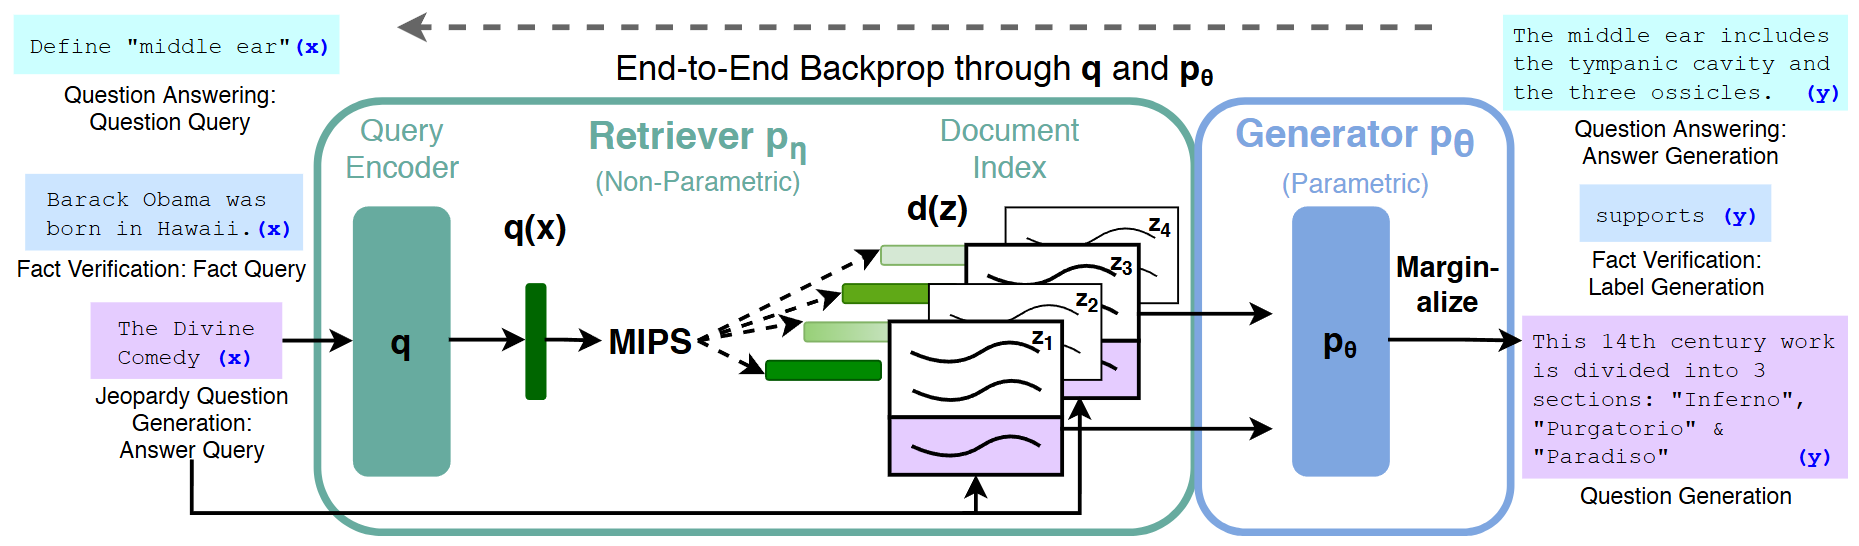
\includegraphics[width=\textwidth]{../images/rag_architecture.png}
    \caption{Overview of the RAG architecture \cite{lewis2021retrievalaugmentedgenerationknowledgeintensivenlp}. For finding the top-k documents $z_i$, the authors used Maximum Inner Product Search (MIPS).}\label{fig:rag_architecture}
\end{figure}

By using an external retrieval corpus, the knowledge RAG models use to inform their generation can directly be inspected and interpreted \cite{lewis2021retrievalaugmentedgenerationknowledgeintensivenlp}. Their TODO

% special challenges of scientific text (short)

% why bother with citations
citations build trust \cite{do2024facilitatinghumanllmcollaborationfactuality}
% hallucinations
% interpretability
% provenance
% ...